\section{React} 

\subsection{Overview}
React is a JavaScript library, based on npm and made by Facebook, for building user intrerfaces by assembling user-defined components.
\subsection{Components}
Components are the key of this npm module, \textit{Soldino} is made by two types of component:
\begin{itemize}
	\item Presentational components;
	\item Container components.
\end{itemize}
\subsubsection{Presentational}
Each presentational component implements \textit{Component} interface provided by the library. According to this interface, some methods are inherited to the presentational components, in particular our components uses \textit{Render()} method for rendering themselves.
Most components can be customized when they are created, with different parameters. These creation parameters are called \textit{props}. Each presentational component returns a single HTML tag, here we can customize the returned tag with some Bootstrap classes. The props are accessible, by components which own them, referencing to them with \textit{this.props.propsName}.

\subsubsection{Containers} 
This type of component is like a wrapper of presentational components. A function called \textit{Connect(arg1, arg2)} is needed for connecting a container component to a presentational component, in this way we are able to map inside the presentational component some actions and some application state variables passing them through props. The \textit{arg1} is a function called \textit{mapStateToProps()} and the \textit{arg2} is another function called \textit{mapDispatchToProps()}.
\subsection{React-Router} 
React-router-dom is a npm module used for rendering different pages without reloading the entire website, this module works with \textit{Render()} method provided by each presentational component. \textit{Soldino} is a single page application, so the router, implemented into a JavaScript file called \textit{App.js}, is responsible to manage which components should be rendered.

\subsection{UML} 
\begin{figure}[H]
	\centering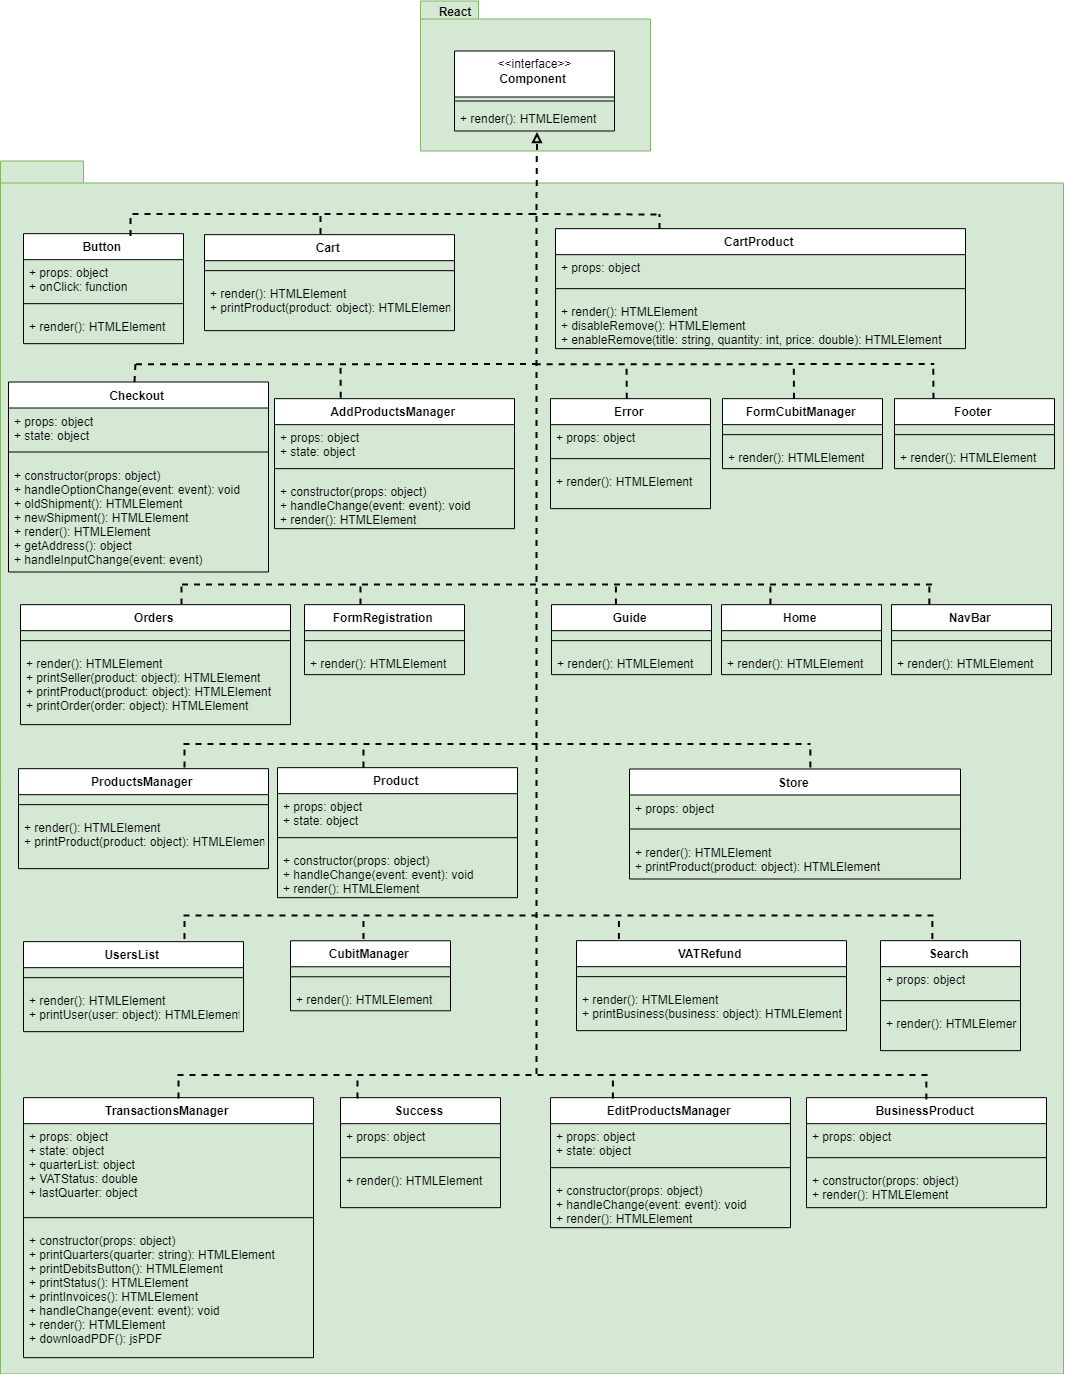
\includegraphics[scale = 0.38]{res/images/Presentational.png}
	\caption{Presentational components}
\end{figure}
\begin{figure}[H]
	\centering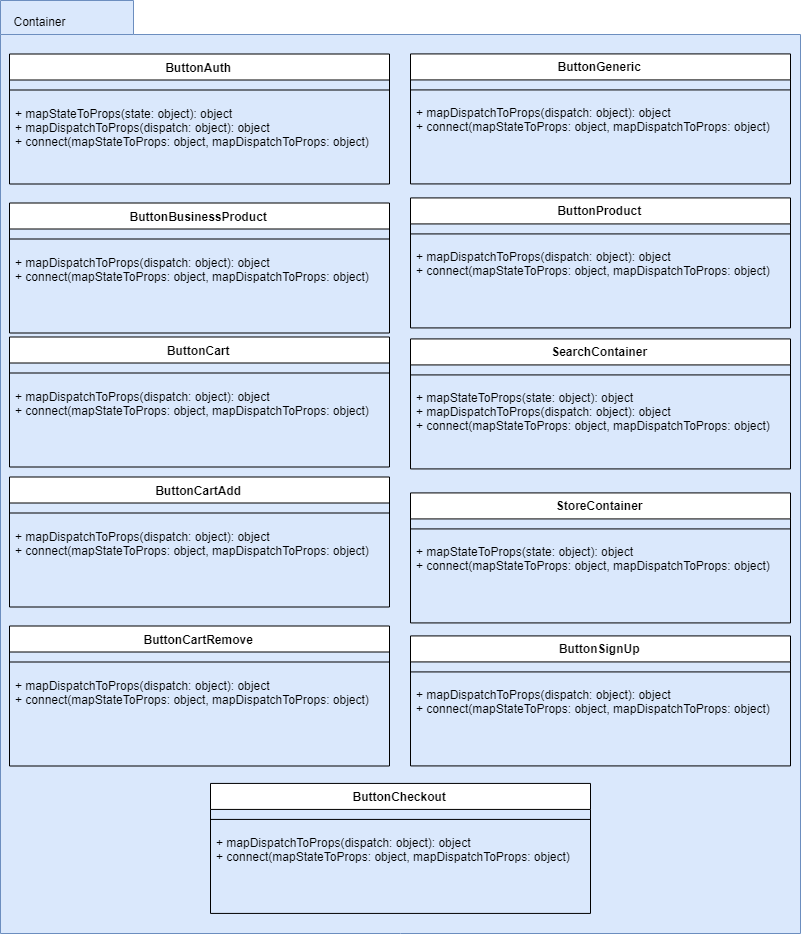
\includegraphics[scale = 0.5]{res/images/Container.png}
	\caption{Container components}
\end{figure}
% \subsection{Collaborations % } if there is one, sequence diag
% \subsection{How to extend} Super optional
